% Laboratorio MAS · Guía del estudiante. Compilar con: tectonic manual_estudiante.tex
\documentclass[11pt,a4paper]{article}
\usepackage[spanish,es-noshorthands,es-nodecimaldot,es-tabla]{babel}
\usepackage{fontspec}
\usepackage[margin=2.2cm,top=2.4cm]{geometry}
\usepackage{amsmath,amssymb}
\usepackage{graphicx,booktabs,tabularx,array,enumitem,multicol}
\usepackage{xcolor}
\usepackage{tikz}
\usetikzlibrary{arrows.meta,positioning,shapes.geometric,calc}
\usepackage[most]{tcolorbox}
\usepackage[hidelinks]{hyperref}
\usepackage{fancyhdr}
\graphicspath{{img/}}
\setlength{\parskip}{5pt}\setlength{\parindent}{0pt}
\setlist{itemsep=2pt,topsep=3pt}

% --- colores de la app ---
\definecolor{acento}{HTML}{2457C5}
\definecolor{acentof}{HTML}{E8EEFB}
\definecolor{ok}{HTML}{1D7A4F}
\definecolor{okf}{HTML}{E6F4EC}
\definecolor{mal}{HTML}{B42318}
\definecolor{malf}{HTML}{FDECEA}
\definecolor{aviso}{HTML}{A15C07}
\definecolor{avisof}{HTML}{FDF3E2}
\definecolor{tinta}{HTML}{17202B}
\definecolor{suave}{HTML}{5B6675}

\hypersetup{colorlinks=true,urlcolor=acento,linkcolor=acento}
\newtcolorbox{idea}[1][Idea clave]{colback=acentof,colframe=acento,fonttitle=\bfseries,title={#1},boxrule=.6pt,arc=2mm}
\newtcolorbox{ojo}[1][Ojo]{colback=malf,colframe=mal,fonttitle=\bfseries,title={#1},boxrule=.6pt,arc=2mm}
\newtcolorbox{consejo}[1][Consejo]{colback=okf,colframe=ok,fonttitle=\bfseries,title={#1},boxrule=.6pt,arc=2mm}
\newtcolorbox{nota}[1][]{colback=avisof,colframe=aviso,fonttitle=\bfseries,title={#1},boxrule=.6pt,arc=2mm}
\newtcolorbox{formula}{colback=white,colframe=acento!50,boxrule=.5pt,arc=1mm}
\newcommand{\boton}[1]{\tikz[baseline=(b.base)]\node[draw=acento,fill=acento,text=white,rounded corners=2pt,inner sep=2.5pt,font=\small\bfseries](b){#1};}
\newcommand{\pestana}[1]{\textbf{\textcolor{acento}{#1}}}
\newcommand{\captura}[2][1060]{\includegraphics[width=\linewidth,trim=0 #1 0 0,clip]{#2}}

\newcommand{\autor}{Francisco Orbe}   % nombre que aparece en todas las páginas
\pagestyle{fancy}\fancyhf{}
\lhead{\small\textcolor{suave}{Laboratorio MAS · Guía del estudiante}}
\rhead{\small\textcolor{suave}{\thepage}}
\cfoot{\small\textcolor{suave}{\autor}}
\renewcommand{\headrulewidth}{0.3pt}
\fancypagestyle{plain}{\fancyhf{}\cfoot{\small\textcolor{suave}{\autor}}\renewcommand{\headrulewidth}{0pt}}

\begin{document}

% ================= PORTADA =================
\begin{titlepage}
\centering
\vspace*{1.5cm}
\begin{tikzpicture}
  % resorte y bloque
  \draw[line width=3pt,acento] (0,0) -- (0,2.2);
  \draw[line width=1.6pt,suave] (0,1.1) -- (0.5,1.1) -- (0.75,1.55) -- (1.25,0.65) -- (1.75,1.55) -- (2.25,0.65) -- (2.75,1.55) -- (3.25,0.65) -- (3.75,1.55) -- (4.0,1.1) -- (4.5,1.1);
  \fill[acento,rounded corners=4pt] (4.5,0.35) rectangle (6.0,1.85);
  \node[white,font=\bfseries\Large] at (5.25,1.1) {m};
  \draw[line width=1pt,suave] (-0.3,0.3) -- (7,0.3);
\end{tikzpicture}

\vspace{1.2cm}
{\Huge\bfseries Laboratorio \textcolor{acento}{MAS}\par}
\vspace{0.4cm}
{\Large Guía del estudiante\par}
\vspace{0.8cm}
{\large ¿Es un movimiento armónico simple?\\ Investiga un sistema masa-resorte con mediciones, predicciones y razonamiento\par}
\vspace{1.5cm}
\begin{tcolorbox}[colback=acentof,colframe=acento,width=.75\textwidth,halign=center,arc=2mm]
\large Enlace de la aplicación\\[3pt]
\Large\bfseries\url{https://theoreticallab.github.io/}
\end{tcolorbox}
\vspace{1cm}
{\normalsize Funciona en el móvil y en el ordenador · sin registro · sin instalar nada\par}
\vfill
{\large \autor\par}
\vspace{2pt}
{\small\textcolor{suave}{Física General}\par}
\end{titlepage}

\tableofcontents
\newpage

% ================= 1 =================
\section{Qué vas a hacer}

En este laboratorio no hay una respuesta que copiar: hay un sistema que investigar. Tienes seis experimentos, llamados \textbf{A, B, C, D, E e I}. En cada uno, un bloque de masa $m$ unido a un resorte horizontal de constante $k$ se suelta desde $x = A$ (estirado) y sin velocidad.

Tu misión en cada experimento es \textbf{decidir, con tus mediciones y tu razonamiento, si el movimiento es compatible con el movimiento armónico simple (MAS) ideal} que predicen los parámetros nominales $m$, $k$ y $A$ que te da la aplicación.

Al final eliges una de tres conclusiones:

\begin{center}
\begin{tabular}{lp{10.5cm}}
\toprule
\textbf{Compatible con el MAS ideal} & Tus datos no contradicen el MAS ideal dentro de su incertidumbre. \\
\textbf{Incompatible con el MAS ideal} & Tienes al menos una discrepancia clara y significativa. \\
\textbf{Evidencia insuficiente} & Con lo que mediste no se puede decidir con honestidad. \\
\bottomrule
\end{tabular}
\end{center}

\begin{idea}
\textbf{«Compatible» no significa «demostrado».} Ninguna medición tiene precisión infinita: lo más que puedes afirmar es que tus datos no contradicen una hipótesis. Reconocer los límites de tus mediciones está bien visto en la nota. Lo que no se valora es acertar por casualidad sin evidencia.
\end{idea}

Cada estudiante recibe experimentos \textbf{distintos}. Aunque tú y tu compañero elijáis la misma letra, tendréis otros números y quizá otro sistema. Podéis comentar ideas, pero los datos y las conclusiones son de cada uno.

% ================= 2 =================
\section{Antes de empezar}

\subsection{Tu identificador}
Al pulsar \boton{Empezar investigación} la aplicación te asigna un identificador con la forma \texttt{MAS-XXXX-XXXX}. \textbf{Anótalo.} Con él tu profesor puede reproducir exactamente tus experimentos, y tú puedes volver a abrir los mismos sistemas si algo falla.

\subsection{Dónde se guarda tu trabajo}
\begin{ojo}[Tu progreso se guarda solo en ese navegador]
\begin{itemize}
\item Trabaja siempre en el \textbf{mismo dispositivo y el mismo navegador}.
\item No uses el \textbf{modo incógnito} ni borres los datos de navegación: perderías lo que hiciste.
\item Si cambias de móvil, con tu identificador recuperas los mismos experimentos, pero no lo que ya habías medido.
\end{itemize}
\end{ojo}

\subsection{Reglas éticas y registro de integridad}
El trabajo es \textbf{individual} y debes responder \textbf{sin inteligencia artificial ni ayuda externa}, razonando con tus propias mediciones. La aplicación lo apoya de forma transparente:

\begin{itemize}
\item \textbf{No se puede pegar texto} en ningún campo. Tampoco funcionan los bloques de texto del portapapeles del teclado ni el dictado de frases enteras: escribe tus respuestas tú.
\item Se \textbf{registra cada vez que sales de la aplicación} (a otra app o pestaña) y cuánto tiempo, sobre todo si estabas respondiendo una pregunta, una predicción o tu conclusión. Al volver aparece un aviso con las reglas.
\item También se registra si \textbf{copias el enunciado} de una pregunta y \textbf{cómo escribes} tus respuestas.
\item Tus pantallas llevan una \textbf{marca de agua} con tu identificador y tu alias.
\end{itemize}
Tu profesor verá ese registro junto a tu informe. No resta puntos automáticamente, pero sirve para valorar tu trabajo.

\begin{center}
\begin{minipage}{.30\textwidth}\centering
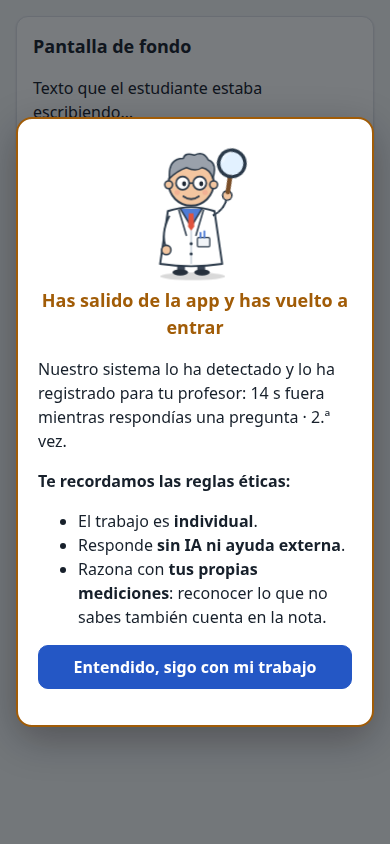
\includegraphics[width=\linewidth]{emergente_claro_400.png}\\[2pt]
{\small\textcolor{suave}{Aviso al volver a la aplicación.}}
\end{minipage}
\end{center}

\begin{consejo}[Si te llaman o te llega un mensaje]
No pasa nada: atiéndelo y vuelve. Un registro aislado no significa nada. Lo que importa es tu razonamiento, y ese solo puedes construirlo tú con tus datos.
\end{consejo}

% ================= 3 =================
\section{Recorrido por la aplicación}

La aplicación tiene cinco pantallas. En el móvil están en la barra inferior y en el ordenador en la superior: \pestana{Inicio}, \pestana{Laboratorio}, \pestana{Instrumentos}, \pestana{Investigación} e \pestana{Informe}. En la cabecera ves siempre tu identificador, el experimento abierto y tus créditos.

\subsection{Inicio: elige un experimento}
\begin{minipage}[t]{.27\textwidth}\vspace{0pt}\captura[1290]{inicio_movil.png}\end{minipage}\hfill
\begin{minipage}[t]{.68\textwidth}\vspace{0pt}
\begin{enumerate}
\item Escribe tu nombre o alias (aparece en tu informe) y pulsa \boton{Empezar investigación}.
\item Toca una letra para abrir ese experimento. Tu profesor te dirá cuáles hacer.
\item Cada tarjeta muestra si el experimento está sin empezar, en curso (con los créditos que te quedan) o entregado.
\item Cada experimento tiene sus propios \textbf{32 créditos}.
\end{enumerate}
\textbf{Continuar o reproducir:} si tienes un identificador anterior, escríbelo para abrir esos mismos experimentos.
\end{minipage}

\subsection{Laboratorio: observa el sistema}
\begin{minipage}[t]{.27\textwidth}\vspace{0pt}\captura[1240]{laboratorio_movil.png}\end{minipage}\hfill
\begin{minipage}[t]{.68\textwidth}\vspace{0pt}
\begin{itemize}
\item \boton{Observar} reproduce el movimiento. Puedes ir más despacio (×0,5, ×0,25) o volver a $t=0$.
\item La animación muestra \emph{cómo} se mueve, no los valores. \textbf{Los números se obtienen midiendo.}
\item Con el deslizador eliges un instante entre 0 y 60\,s, y \boton{Medir en t = …} lo lleva a Instrumentos.
\item \textbf{Montaje actual:} los parámetros nominales $m$, $k$ y $A$ con los que harás tus predicciones.
\item \textbf{Cambiar el montaje:} puedes montar el bloque con el doble o la mitad de masa, o soltarlo con el doble o la mitad de amplitud. Cada configuración nueva cuesta 3 créditos una sola vez; volver a una ya montada es gratis. El resorte es siempre el mismo.
\item \textbf{Formulario del MAS ideal:} ábrelo cuando lo necesites.
\end{itemize}
\end{minipage}

\subsection{Instrumentos: predice y mide}
\begin{minipage}[t]{.27\textwidth}\vspace{0pt}\captura[1340]{instrumentos_movil.png}\end{minipage}\hfill
\begin{minipage}[t]{.68\textwidth}\vspace{0pt}
Cada medición sigue estos pasos:
\begin{enumerate}
\item \textbf{Elige el instrumento} y sus datos (instante, número de oscilaciones, posición…). Verás el coste antes de gastar nada.
\item Pulsa \boton{Solicitar}.
\item \textbf{Escribe tu predicción} según el MAS ideal con los parámetros nominales, en las unidades indicadas, y una justificación breve (la fórmula que usas).
\item \boton{Confirmar predicción}. \textbf{Ya no se puede cambiar.}
\item \boton{Realizar la medición}: obtienes el valor con su incertidumbre y la comparación con tu predicción.
\end{enumerate}
\textbf{Repetir} una medición idéntica no pide predicción. Da otro valor, porque el instrumento tiene ruido, pero el valor verdadero es el mismo.
\end{minipage}

\vspace{6pt}
\begin{center}
\begin{tabular}{lcp{8.6cm}}
\toprule
\textbf{Instrumento} & \textbf{Créditos} & \textbf{Qué mide} \\
\midrule
Posición & 1 & $x$ en el instante $t$ \\
Velocidad & 2 & $v$ en el instante $t$ \\
Aceleración & 2 & $a$ en el instante $t$ \\
Fuerza del resorte & 2 & Fuerza que el resorte ejerce sobre el bloque en $t$ \\
Energía & 3 & Energía cinética $K$, potencial $U$ y mecánica $E$ en $t$ \\
Período (cronómetro) & 2 / 3 / 4 & Cronometra 1, 5 o 10 oscilaciones desde $t=0$ \\
Frecuencia & 3 & Frecuencia de oscilación con un frecuencímetro \\
Aceleración en una posición & 3 & $a$ la primera vez que el bloque pasa por $x$ (de $+A$ hacia $-A$) \\
Registro de posición & 6 & $x$ en 10 instantes equiespaciados entre $t_1$ y $t_2$ \\
Montaje nuevo & 3 & Cambiar masa o amplitud (una vez por configuración) \\
\bottomrule
\end{tabular}
\end{center}

En el \textbf{registro de mediciones}, junto a cada predicción aparece un número seguido de $\sigma$: cuántas incertidumbres separan tu predicción de lo medido (ver sección~\ref{sec:z}). Las \textbf{gráficas} se dibujan solo con los datos que tú hayas medido, con sus barras de error, y tus predicciones aparecen como círculos huecos.

\subsection{Investigación: preguntas e hipótesis}
\begin{minipage}[t]{.27\textwidth}\vspace{0pt}\captura[1260]{investigacion_movil.png}\end{minipage}\hfill
\begin{minipage}[t]{.68\textwidth}\vspace{0pt}
\textbf{Preguntas.} No son una lista fija: dependen de lo que mides, predices y respondes, y usan \textbf{tus propios números}. Las hay de tres tipos:
\begin{itemize}
\item \emph{Cálculo:} un número con su unidad, con tolerancia.
\item \emph{Razonamiento:} eliges la opción que mejor se apoya en tus datos.
\item \emph{Reflexión:} explicas tu decisión por escrito; la revisa tu profesor.
\end{itemize}
Después de responder verás si tu razonamiento es coherente con tus datos. \boton{Ahora no} pospone una pregunta: puede volver si cambia tu evidencia.

\textbf{Hipótesis.} Valora cada hipótesis como \emph{sin evaluar}, \emph{compatible}, \emph{descartada} o \emph{indecidible}. Añade una nota explicando por qué y marca las mediciones en que te apoyas. Cada cambio queda registrado: \textbf{revisar una hipótesis ante nueva evidencia es buen trabajo científico}, no un error.
\end{minipage}

\subsection{Informe: concluye y entrega}
\begin{minipage}[t]{.27\textwidth}\vspace{0pt}\captura[1200]{informe_movil.png}\end{minipage}\hfill
\begin{minipage}[t]{.68\textwidth}\vspace{0pt}
\begin{enumerate}
\item Elige una conclusión y pulsa \boton{Proponer esta conclusión}.
\item En \pestana{Investigación} aparecerá una \textbf{pregunta de desafío} sobre tu conclusión. Respóndela con calma; puedes cambiar de conclusión hasta entregar.
\item Rellena la entrega final:
  \begin{itemize}
  \item las \textbf{mediciones} que sostienen tu conclusión;
  \item la \textbf{significación} $z$ de tu evidencia principal (opcional, pero suma);
  \item las \textbf{limitaciones} que reconoces;
  \item una \textbf{justificación}: qué mediste, qué esperabas, qué observaste y con qué significación.
  \end{itemize}
\item \boton{Entregar (definitivo)}: ya no podrás medir ni cambiar respuestas.
\end{enumerate}
Después verás tu \textbf{calificación provisional}, que tu profesor revisará, y podrás enviar o descargar tu informe (sección~\ref{sec:entrega}).
\end{minipage}

\begin{consejo}[Siempre puedes terminar]
Aunque te quedes sin créditos o sin mediciones, siempre puedes entregar declarando que la evidencia es insuficiente y explicando qué medirías para decidir.
\end{consejo}

% ================= 4 =================
\section{La física y la estadística que necesitas}

No hace falta cálculo diferencial: basta con estas fórmulas, cocientes, medias y la comparación $z$.

\subsection{El MAS ideal}
Con $x(0)=A$ y $v(0)=0$:
\begin{formula}
\begin{minipage}{.48\linewidth}
\begin{align*}
x(t) &= A\cos(\omega t) \\
v(t) &= -A\,\omega\sin(\omega t) \\
a(t) &= -\omega^2\,x(t) \\
F(t) &= -k\,x(t)
\end{align*}
\end{minipage}\hfill
\begin{minipage}{.48\linewidth}
\begin{align*}
\omega &= \sqrt{k/m}, \quad T = 2\pi\sqrt{m/k}, \quad f = 1/T \\
v_{\max} &= A\,\omega, \qquad a_{\max} = A\,\omega^2 \\
K &= \tfrac12 m v^2, \qquad U = \tfrac12 k x^2 \\
E &= K + U = \tfrac12 k A^2
\end{align*}
\end{minipage}
\end{formula}

\begin{ojo}[Errores típicos al predecir]
\begin{itemize}
\item La calculadora debe estar en \textbf{radianes}: $\omega t$ es un ángulo en radianes.
\item $\omega$ se mide en rad/s; $f = \omega/2\pi$ en Hz. No las confundas.
\item Cuida el \textbf{signo}: la velocidad es negativa justo después de soltar el bloque, porque va hacia $-A$.
\item Usa los parámetros del \textbf{montaje actual}: si cambiaste masa o amplitud, cambian tus predicciones.
\end{itemize}
\end{ojo}

\subsection{Incertidumbre y significación $z$}\label{sec:z}
Cada medición viene como \emph{valor} $\pm\ \sigma$, donde $\sigma$ es la incertidumbre típica del instrumento. Para saber si una diferencia es real o es ruido se calcula
\[
z = \frac{\text{observado} - \text{esperado}}{\sigma}.
\]
\begin{center}
\begin{tabular}{lll}
\toprule
$|z| < 2$ & \textcolor{ok}{\textbf{compatible}} & La diferencia cabe en el ruido de la medición. \\
$2 \le |z| < 3$ & \textcolor{aviso}{\textbf{dudoso}} & No decidas todavía: repite o mejora la precisión. \\
$|z| \ge 3$ & \textcolor{mal}{\textbf{significativo}} & Diferencia real muy probable (mejor si la confirmas). \\
\bottomrule
\end{tabular}
\end{center}

Si comparas \textbf{dos mediciones} entre sí, por ejemplo la misma magnitud en dos instantes, usa
\[
z = \frac{x_2 - x_1}{\sqrt{\sigma_1^2+\sigma_2^2}}.
\]

\begin{idea}[Cuidado con las comparaciones múltiples]
Si haces muchas mediciones, alguna puede salir a $3\sigma$ por puro azar. Una sola discrepancia aislada no basta: confírmala repitiendo antes de concluir.
\end{idea}

\subsection{Repetir y promediar}
Si repites $n$ veces la misma medición:
\[
\bar{x} = \frac{1}{n}\sum x_i, \qquad s = \sqrt{\frac{\sum (x_i-\bar x)^2}{n-1}}, \qquad \sigma_{\bar x} = \frac{\sigma}{\sqrt{n}}.
\]
Promediar reduce la incertidumbre, pero cuesta créditos. Para el período hay un truco más barato: cronometrar \textbf{10 oscilaciones} y dividir entre 10 reduce el error del cronómetro a la décima parte por solo 4 créditos.

\subsection{Cocientes}
Para comparar dos períodos (por ejemplo, con distinta masa o amplitud), calcula el cociente $r = T_2/T_1$ y su incertidumbre:
\[
\sigma_r = r\sqrt{\left(\frac{\sigma_{T_1}}{T_1}\right)^2 + \left(\frac{\sigma_{T_2}}{T_2}\right)^2}.
\]
Después compara $r$ con lo que predice el MAS ideal mediante $z$.

% ================= 5 =================
\section{Cómo planificar tu investigación}

\begin{center}
\begin{tikzpicture}[node distance=7mm and 9mm,caja/.style={draw=acento,fill=acentof,rounded corners=3pt,minimum width=2.4cm,minimum height=9mm,align=center,font=\small},>=Stealth]
\node[caja] (h) {Hipótesis};
\node[caja,right=of h] (p) {Predicción\\(MAS ideal)};
\node[caja,right=of p] (m) {Medición};
\node[caja,right=of m] (c) {Comparación\\($z$)};
\node[caja,below=of m] (r) {Revisar\\hipótesis};
\draw[->,thick,acento] (h) -- (p); \draw[->,thick,acento] (p) -- (m); \draw[->,thick,acento] (m) -- (c);
\draw[->,thick,acento] (c) |- (r); \draw[->,thick,acento] (r) -| (h);
\end{tikzpicture}
\end{center}

\begin{enumerate}
\item \textbf{Empieza calculando.} Con $m$, $k$ y $A$ nominales, calcula $\omega$, $T$, $v_{\max}$ y $E$. Las primeras preguntas te lo pedirán.
\item \textbf{Formula hipótesis rivales.} No basta con «es un MAS». Pregúntate qué otras explicaciones darían resultados parecidos. La pantalla Investigación lista varias.
\item \textbf{Elige mediciones que distingan.} Antes de gastar créditos pregúntate: \emph{¿qué resultado esperaría si fuera un MAS ideal, y qué resultado si fuera cada alternativa?} Si las dos hipótesis predicen lo mismo, esa medición no te ayuda a decidir entre ellas.
\item \textbf{Piensa en el tiempo y en las condiciones.} Algunas diferencias solo aparecen comparando instantes muy separados, o cambiando la masa o la amplitud del montaje.
\item \textbf{Repite lo dudoso,} no lo que ya está claro.
\item \textbf{Actualiza tus hipótesis} cada vez que aparezca evidencia nueva, y deja escrito el porqué.
\item \textbf{Concluye con honestidad:} ni más fuerte ni más débil de lo que dicen tus datos.
\end{enumerate}

\subsection*{Hoja de planificación (rellénala antes de medir)}
\begin{center}
\renewcommand{\arraystretch}{1.6}
\begin{tabularx}{\textwidth}{|p{3.3cm}|X|X|c|}
\hline
\textbf{Medición} & \textbf{Si es MAS ideal espero…} & \textbf{Si es otra hipótesis espero…} & \textbf{Créditos} \\ \hline
 & & & \\ \hline
 & & & \\ \hline
 & & & \\ \hline
 & & & \\ \hline
\multicolumn{3}{|r|}{\textbf{Total (máximo 32)}} & \\ \hline
\end{tabularx}
\end{center}

% ================= 6 =================
\section{Ejemplo resuelto (con números inventados)}

Supón un montaje con $m = 0{,}50$\,kg, $k = 20$\,N/m y $A = 0{,}10$\,m. Tus números serán otros.

\textbf{1. Cálculos previos.}
\begin{align*}
\omega &= \sqrt{\frac{20}{0{,}50}} = 6{,}32\ \text{rad/s}, & T &= \frac{2\pi}{\omega} = 0{,}993\ \text{s},\\
v_{\max} &= A\,\omega = 0{,}632\ \text{m/s}, & E &= \tfrac12\,(20)(0{,}10)^2 = 0{,}100\ \text{J}.
\end{align*}

\textbf{2. Una predicción.} Posición en $t = 3{,}00$\,s:
\[
x(3) = 0{,}10\,\cos(6{,}325\times 3{,}00) = 0{,}10\,\cos(18{,}97\ \text{rad}) = 0{,}10\times 0{,}992 = 0{,}0992\ \text{m}.
\]
Justificación que escribirías: «$x = A\cos(\omega t)$ con $\omega=\sqrt{k/m}$, calculadora en radianes».

\textbf{3. Comparar con la medición.} Supón que el cronómetro de 10 oscilaciones da $T = 1{,}012 \pm 0{,}008$\,s:
\[
z = \frac{1{,}012 - 0{,}993}{0{,}008} = 2{,}4 \quad\Rightarrow\quad \text{dudoso: todavía no concluyas.}
\]
¿Qué harías? Repetir mejora la precisión. Pero piensa también: si la diferencia fuera real, ¿qué hipótesis la explicarían, y qué otra medición las distinguiría entre sí?

\textbf{4. Promediar.} Tres mediciones de posición en el mismo instante: $0{,}0981$, $0{,}1004$, $0{,}0987$\,m con $\sigma = 0{,}0015$\,m:
\[
\bar x = 0{,}0991\ \text{m},\qquad \sigma_{\bar x} = \frac{0{,}0015}{\sqrt 3} = 0{,}0009\ \text{m},\qquad
z = \frac{0{,}0991 - 0{,}0992}{0{,}0009} = -0{,}1 \Rightarrow \text{compatible.}
\]

% ================= 7 =================
\section{Cómo se evalúa}

La nota (sobre 100) tiene cinco partes de 20 puntos:

\begin{center}
\begin{tabularx}{\textwidth}{lX}
\toprule
\textbf{Predicciones} & Aplicar bien el MAS ideal \emph{antes} de medir, con una justificación. Se compara con el cálculo correcto, no con lo que salió. \\
\textbf{Selección de experimentos} & Elegir mediciones que de verdad distingan entre hipótesis y usar bien el presupuesto. \\
\textbf{Cálculos} & Las preguntas numéricas (con tolerancia) y la significación $z$ de tu conclusión. \\
\textbf{Razonamiento} & Las preguntas de razonamiento, la revisión fundamentada de tus hipótesis y corregir tus propios errores. \\
\textbf{Conclusión} & Que tu conclusión esté justificada con \emph{tus} datos y que reconozcas sus limitaciones. Acertar sin evidencia vale poco; declarar «evidencia insuficiente» cuando de verdad lo es, vale mucho. \\
\bottomrule
\end{tabularx}
\end{center}

La nota que ves al entregar es \textbf{automática y provisional}. Tu profesor revisa tus textos (justificaciones, explicaciones, conclusión) y puede ajustarla.

% ================= 8 =================
\section{Cómo entregar}\label{sec:entrega}

Después de pulsar \boton{Entregar (definitivo)}, en la pantalla \pestana{Informe}:

\begin{itemize}
\item \textbf{Si ves el botón \boton{Enviar al profesor}:} escribe el \textbf{código de clase} que te dé tu profesor y pulsa enviar. Recibirás un \textbf{recibo} de 6 caracteres; guárdalo como comprobante.
\item \textbf{Si no aparece} (o el envío falla): pulsa \boton{Descargar informe (HTML)} y \boton{Descargar datos (JSON)} y entrega \textbf{los dos archivos} como indique tu profesor. Sin el JSON no se puede revisar tu investigación.
\end{itemize}

\begin{nota}[Fecha límite]
Entrega antes de: \rule{6cm}{0.4pt}\qquad Código de clase: \rule{3cm}{0.4pt}
\end{nota}

% ================= 9 =================
\section{Preguntas frecuentes}

\begin{description}[style=nextline,leftmargin=0pt,itemsep=6pt]
\item[He cerrado la aplicación. ¿Perdí todo?] No: al volver a abrirla en el mismo navegador sigue donde estabas. Solo se pierde si usas modo incógnito, borras los datos de navegación o cambias de dispositivo.
\item[Cambié de móvil.] Escribe tu identificador en \emph{Continuar o reproducir}: tendrás los mismos experimentos, pero tendrás que volver a medir.
\item[Me he quedado sin créditos.] Puedes seguir respondiendo preguntas, ajustar tus hipótesis y entregar. Si tu evidencia no basta, declara «evidencia insuficiente» y explica qué medirías.
\item[No puedo pegar texto.] Es intencionado: escribe tus respuestas tú. El dictado de frases enteras también se bloquea.
\item[Me salió el aviso «Has salido de la app».] Es un recordatorio. Si fue una llamada o un mensaje, pulsa \emph{Entendido} y sigue trabajando.
\item[No entiendo una pregunta.] Relee tus mediciones y el formulario. Puedes pulsar \emph{Ahora no} y volver más tarde, o preguntar a tu profesor.
\item[Mi compañero tiene números distintos.] Es normal: cada estudiante tiene sus propios experimentos.
\item[Me equivoqué en una predicción.] Ya no se puede cambiar, pero puedes revisar tu interpretación y, si te lo preguntan, recalcularla. Corregir tus errores con fundamento también suma.
\item[¿Puedo hacer varios experimentos?] Sí, cada uno con sus 32 créditos y su propia entrega.
\end{description}

% ================= 10 =================
\section{Lista de comprobación antes de entregar}

\begin{itemize}[label=$\square$,itemsep=4pt]
\item Anoté mi identificador.
\item Calculé las predicciones del MAS ideal con los parámetros del montaje que usé.
\item Mis predicciones tienen una justificación (fórmula o razonamiento).
\item Elegí mediciones que distinguen entre hipótesis, no solo las que confirman la mía.
\item Repetí las mediciones dudosas ($2\le|z|<3$).
\item Revisé mis hipótesis y escribí por qué las cambié.
\item Respondí la pregunta de desafío de mi conclusión.
\item Mi conclusión cita las mediciones que la sostienen, su $z$ y sus limitaciones.
\item Envié mi investigación (y guardé el recibo) o descargué los dos archivos y los entregué.
\end{itemize}

\vfill
\begin{center}\small\textcolor{suave}{Laboratorio MAS · \url{https://theoreticallab.github.io/}}\end{center}

\end{document}
